\documentclass{article}

% Configurações Genéricas ------------------------------------------------------
\usepackage[utf8]{inputenc}
\usepackage[T1]{fontenc}
\usepackage[brazil]{babel}
\usepackage{sbc-template}
\usepackage{graphicx}

% Informações Pessoais ---------------------------------------------------------
\title{Tarefa 13 sobre Desenvolvimento com Windows Phone 7}
\author{Wanderson Henrique Camargo Rosa\inst{1}}
\address{Programação para Dispositivos Móveis 2011/1\\Centro de Ciências Exatas
e Tecnológicas\\Universidade do Vale do Rio dos Sinos ---
UNISINOS\email{wandersonwhcr@gmail.com}}

% Documento --------------------------------------------------------------------
\begin{document}

\maketitle{}

% Introdução -------------------------------------------------------------------
\section{Introdução}
\label{sec:introducao}

O presente documento é resultado da décima terceira tarefa sobre desenvolvimento
em dispositivos móveis proposta pela disciplina. Há necessidade de criação de um
aplicativo qualquer sobre a plataforma Windows Phone 7. Serão descritos os
problemas encontrados durante a instalação do ambiente de desenvolvimento e a
impossibilidade de construção de qualquer tipo de aplicativo.

A Seção \ref{sec:tentativa} começa a descrever a primeira tentativa de
instalação do ambiente de desenvolvimento sobre o Sistema Operacional Windows
XP. A Seção \ref{sec:programando} apresenta alguns recursos utilizados durante o
início da programação e os primeiros problemas encontrados durante a execução do
emulador. Já a Seção \ref{sec:sistema} relata como foi a troca do Sistema
Operacional para Microsoft Windows 7 Ultimate e a Seção \ref{sec:reinstalacao}
exibe informações sobre a reinstalação do ambiente de desenvolvimento
possivelmente com problemas. Considerações finais sobre análise, opinião pessoal
e tempos decorridos são descritos na Seção \ref{sec:consideracoes}.

% Tentativa de Instalação ------------------------------------------------------
\section{Tentativa de Instalação}
\label{sec:tentativa}

A programação sobre a plataforma Windows Phone 7 utiliza o ambiente de
desenvolvimento Microsoft Visual Studio 2010 Express. Para instalação, segundo
os requisitos mínimos é necessário o Sistema Operacional Microsoft Windows Vista
ou superior.

Como não possuo licença para execução deste \textit{software} fechado, precisei
recorrer a instalações paralelas sobre o Sistema Operacional Microsoft Windows
XP. Após acessar alguns fóruns, descobri que existia a possibilidade de extrair
o conteúdo do instalador e modificar alguns arquivos de configuração,
habilitando a execução sobre a plataforma que eu possuo.

A cópia do instalador oficial do ambiente da Microsoft possui cerca de 4MB. Ao
executá-lo sobre o Windows XP, ele não possibilita a sua execução. Executando o
programa utilizando um parâmetro adicional, foi possível extrair o conteúdo
necessário. Após alterar duas linhas do arquivo de configuração, a instalação
pode ser executada com sucesso.

O programa busca cerca de 423MB em arquivos dos servidores da Microsoft. Após
esperar a finalização da cópia, a própria instalação começou a gerar alguns
erros. Ignorando-os, o ambiente de desenvolvimento pode ser aberto depois da
instalação.

% Programando ------------------------------------------------------------------
\section{Programando}
\label{sec:programando}

Com o ambiente instalado, o próximo passo a ser seguido foi o início da leitura
dos documentos disponibilizados na tarefa. Em primeira impressão, o documento
descreve que as visualizações são construídas em formato XAML, separando assim a
camada de controle. A construção de \textit{interfaces} gráficas parece ser
muito mais interessante do que em outras plataformas, exibindo principalmente as
margens utilizadas durante a movimentação de algum componente disposto na tela.

Aplicando o primeiro código disponível no documento e executando sobre o
emulador, muitos erros adicionais são gerados, semelhantes aos do instalador.
Procurando soluções sobre o mesmo fórum, muitos afirmam que os erros gerados são
gerados pela instalação do ambiente de desenvolvimento sobre uma plataforma não
suportada.

Como garantia, a única atualização disponível de cerca de 123MB foi instalada e
os erros continuaram. Sem outra escolha, a procura por um Sistema Operacional
compatível iniciou-se até finalmente encontrar uma mídia de instalação do
Microsoft Windows 7 Ultimate.

% Mudança de Sistema -----------------------------------------------------------
\section{Mudança de Sistema}
\label{sec:sistema}

Utilizando uma máquina virtual sobre o aplicativo Oracle Virtualbox, o Windows 7
foi instalado com sucesso após algumas horas. A instalação do ambiente pode ser
executada sem erros, porém a cópia dos 423MB em arquivos dos servidores e
123MB de atualizações foram novamente necessárias.

Com estes aplicativos devidamente copiados e instalados, o ambiente de
desenvolvimento pode ser executado com sucesso. Incluindo novamente o código
fonte disponível no documento da tarefa e executando o emulador, este não estava
aparecendo. Após um tempo gasto na descoberta do porquê o problema foi gerado, a
janela responsável pelo emulador foi exibida.

\begin{figure}
    \centering{}
    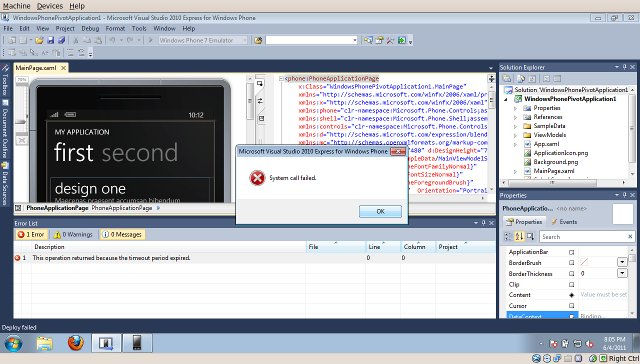
\includegraphics[width=\textwidth]{system-call-failed}
    \caption{Falha em Chamada de Sistema}
    \label{fig:system-call-failed}
\end{figure}

Porém, o emulador não iniciou corretamente. Após cerca de 5 minutos, uma
mensagem de erro informando \textit{timeout} de conexão era exibida ou que uma
\textit{systemcall} era inválida, descrita na Figura
\ref{fig:system-call-failed}.

% Reinstalação -----------------------------------------------------------------
\section{Reinstalação}
\label{sec:reinstalacao}

Novamente pesquisando em fóruns, pessoas afirmam que este problema é solucionado
reinstalando o ambiente de desenvolvimento. Ao acessar o menu \textit{adicionar
ou remover programas} a opção reparar estava disponível. Ao inicializar a
tarefa, o programa novamente efetuou a cópia de instalação proveniente dos
servidores da Microsoft.

Finalizando a reinstalação do ambiente, os códigos inseridos no documento
disponibilizado sempre geravam o mesmo problema, onde o emulador não conseguiu
ser inicializado corretamente, gerando os erros descritos na Seção
\ref{sec:sistema}.

Após esta última tentativa e sem mais idéias sobre soluções, desisti da tarefa
desta semana, gerando o presente relatório descrevendo todos os passos
aplicados.

% Considerações Finais ---------------------------------------------------------
\section{Considerações Finais}
\label{sec:consideracoes}

A criação de ambientes para desenvolvimento em dispositivos móveis pode ser
impossibilitada quando o programador não possui conhecimentos sobre o Sistema
Operacional utilizado. No caso atual, houve uma frustração na tentativa de
criação de um ambiente capaz de facilitar o desenvolvimento para Windows Phone
7.

A utilização de máquinas virtuais para desenvolvimento sempre foi algo simples.
Possíveis testes de execução podem ser utilizados sem a preocupação sobre os
dados armazenados na máquina utilizada. Não existe uma explicação de que esta
utilização foi responsável pelos problemas encontrados.

Em primeiro contato, o ambiente de desenvolvimento Microsfoft Visual Studio 2010
Express parece ter uma \textit{interface} amigável, porém desorganizada. Existem
muitas janelas que podem ser acessadas e esta pode ser uma barreira para
inciantes. Já a construção de visualização utilizando o ambiente é muito
interessante, principalmente na exibição de réguas para posicionamento dos
elementos. Por outro lado, sua utilização pode impedir que a tela seja adaptável
a diferentes tamanhos de dispositivos já que as posições estarão fixadas.

Finalizando, creio que o desenvolvimento sobre a plataforma Windows Phone 7 deve
ser de fácil utilização. A linguagem de programação C\# utilizada é semelhante
ao Java, estrutura pela qual alguns trabalhos já foram desenvolvidos nesta
disciplina. Peço encarecidamente um diálogo sobre este documento, informando um
parecer sobre a impossibilidade de gerar um programa conforme a solicitação da
disciplina.

Para uma primeira análise da tarefa, documentação disponível e inicialização da
instalação do ambiente de desenvolvimento, foram gastas cerca de 2h. A primeira
verificação de erros e inserção do código disponível foram executadas em 30min.
O tempo necessário para conseguir uma mídia de instalação do Microsoft Windows 7
Ultimate não pode ser contabilizada, já que houve uma dependência de terceiros
sobre esta ação. A instalação inicial sobre o novo Sistema demorou cerca de 2h e
as tentativas de busca para solucionar os problemas descritous são
contabilizadas em 10h. Distribuídas entre os dias 31 de maio e 5 de junho de
2011, foram totalizadas cerca de 14h30min para as ações aqui descritas.

\end{document}
